% Design Requirements
\chapter{Design Requirements}

The following requirements are based on the problem statement, team brainstorming, user needfinding, and prototypes. Some of this requirements also come from a geometrical and structural analysis of the plane (cabin and cargo hold) that are detailed in Appendix B.
\\
\\This requirements fall into two categories: Functional and Physical. Functional requirements detail what a design should do, its actions and capabilities. Physical requirements describe the constraints on the manifested system components. 
\\
\\ We have divided the functional and physical requirements into two main parts:
\begin{list}{-}{}
  \item Requirements for the wheelchair platform that will improve wheelchair storage from the jetway to the cargo hold
  \item Requirements for the transfer mechanism that will enable wheelchair passengers to reach their seats in a more comfortable and independent way
\end{list} 

\section{Functional Requirements}

\subsection*{Wheelchair storage device}

In order to prevent wheelchairs from being damaged our team wants to design a platform that will enable baggage handlers to move the mobility device from the jetway to the cargo hold. This platform will be composed of five parts:

\begin{list}{-}{}
  \item A pallet that will support the wheelchair
  \item A moving mechanism to enable transport from jetway to cargo hold
  \item Electronics that will identify who is handling the wheelchair and detect mishandling
  \item A handle that will enable baggage handlers to interact with the platform
  \item A ramp that will enable the wheelchair to be driven on top of the pallet
\end{list}

The functional requirements for each of this part are in the tables from \ref{fig:fun_req_pallet} to \ref{fig:fun_req_ramp}.

\newpage

\begin{figure}[h!]
  \centering
     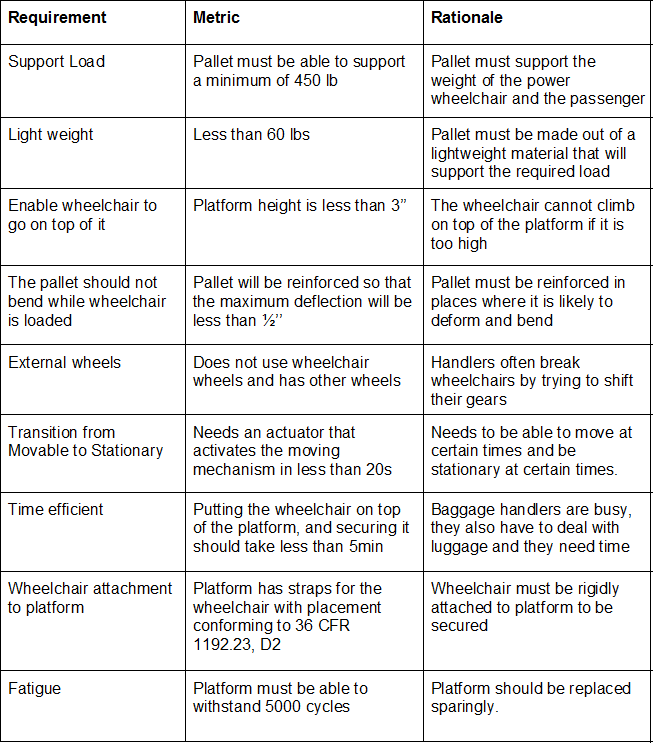
\includegraphics[scale=1]{images/functional_requirements_pallet.png}
   \caption{Functional requirements for the pallet}
  \label{fig:fun_req_pallet}
\end{figure}

\newpage

\begin{figure}[h!]
  \centering
     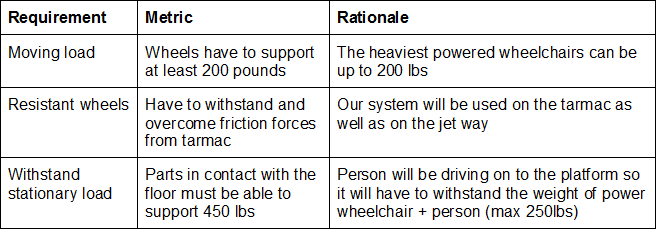
\includegraphics[scale=1]{images/functional_requirements_moving_mechanism.png}
   \caption{Functional requirements for the moving mechanism}
  \label{fig:fun_req_moving_mechanism}
\end{figure}

\newpage

\begin{figure}[h!]
  \centering
     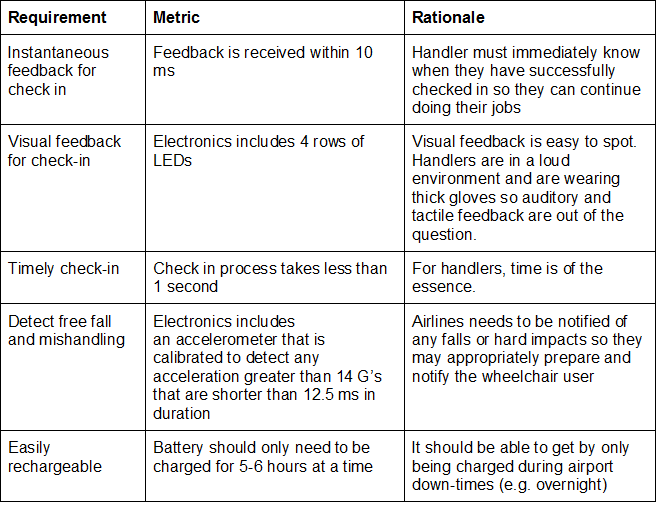
\includegraphics[scale=1]{images/functional_requirements_electronics.png}
   \caption{Functional requirements for the electronics}
  \label{fig:fun_req_electronics}
\end{figure}

\newpage

\begin{figure}[h!]
  \centering
     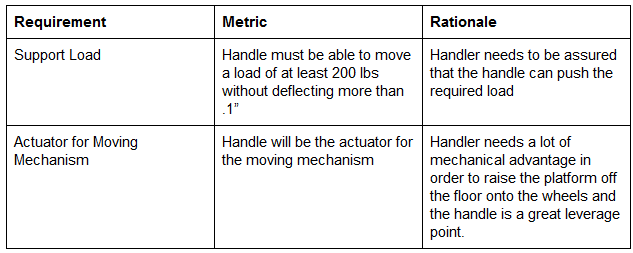
\includegraphics[scale=1]{images/functional_requirements_handle.png}
   \caption{Functional requirements for the handle}
  \label{fig:fun_req_handle}
\end{figure}

\newpage

\begin{figure}[h!]
  \centering
     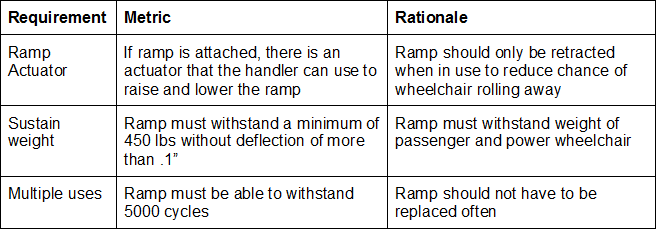
\includegraphics[scale=1]{images/functional_requirements_ramp.png}
   \caption{Functional requirements for the ramp}
  \label{fig:fun_req_ramp}
\end{figure}

\newpage

\subsection*{Wheelchair transfer mechanism}

In order to improve the boarding experience for disabled passengers, our team decided to redesign the aisle wheelchair by making it possible for a wheelchair user to transfer himself from the wheelchair to his seat without needing to be carried by flight attendants. The system that we are designing to give wheelchair users their independence back will be composed of seven parts:

\begin{list}{-}{}
  \item A chest rest that will equip the aisle wheelchair in order to make its use more comfortable and less degrading for passengers
  \item A locomotion mechanism that would enable wheelchair users to move through the cabin
  \item A cushion that will support disabled passengers
  \item A sliding base that will enable transfer from the aisle wheelchair to the airplane seat without external assistance
  \item A wheelchair structure that will completely be redesigned to accomodate the sliding base and the chest rest
  \item A footrest that will enable disabled passengers to have support for their legs
  \item A new airplane seat that will be adapted to the sliding base
\end{list}

The functional requirements for each of this part are in the tables from \ref{fig:fun_req_chest_rest} to \ref{fig:fun_req_airplane_seat}.

\newpage

\begin{figure}[h!]
  \centering
     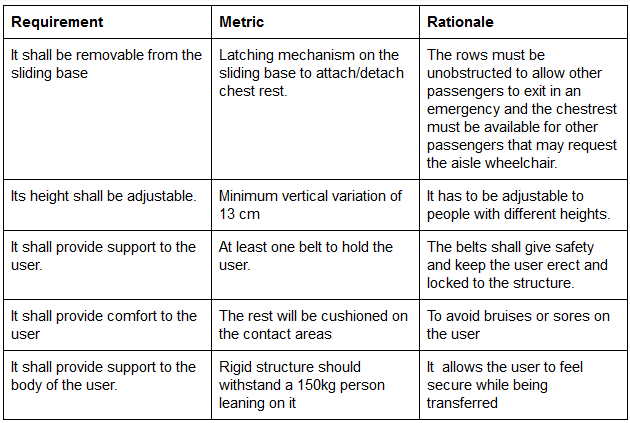
\includegraphics[scale=1]{images/functional_requirements_chest_rest.png}
   \caption{Functional requirements for the chest rest}
  \label{fig:fun_req_chest_rest}
\end{figure}

\newpage

\begin{figure}[h!]
  \centering
     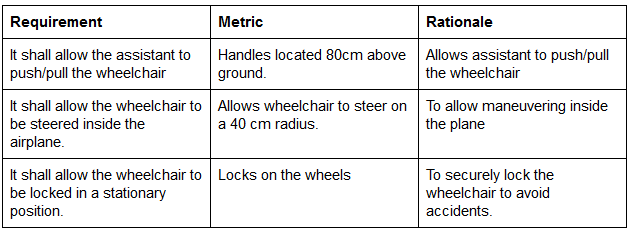
\includegraphics[scale=1]{images/functional_requirements_locomotion_mechanism.png}
   \caption{Functional requirements for the locomotion mechanism}
  \label{fig:fun_req_locomotion_mechanism}
\end{figure}

\newpage

\begin{figure}[h!]
  \centering
     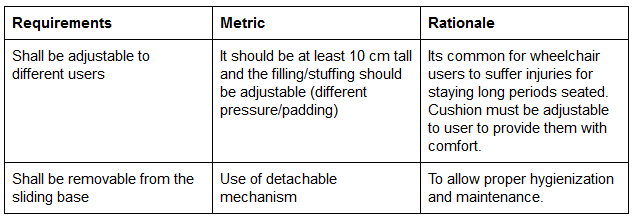
\includegraphics[scale=1]{images/functional_requirements_cushion.png}
   \caption{Functional requirements for the cushion}
  \label{fig:fun_req_cushion}
\end{figure}

\newpage

\begin{figure}[h!]
  \centering
     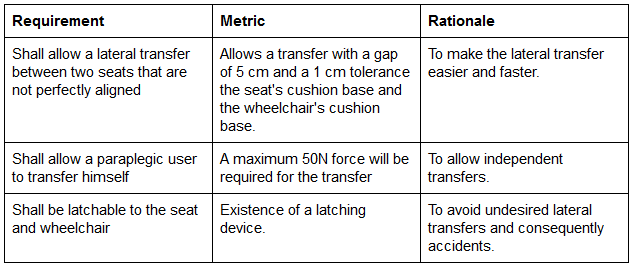
\includegraphics[scale=1]{images/functional_requirements_sliding_base.png}
   \caption{Functional requirements for the sliding base}
  \label{fig:fun_req_sliding_base}
\end{figure}

\newpage

\begin{figure}[h!]
  \centering
     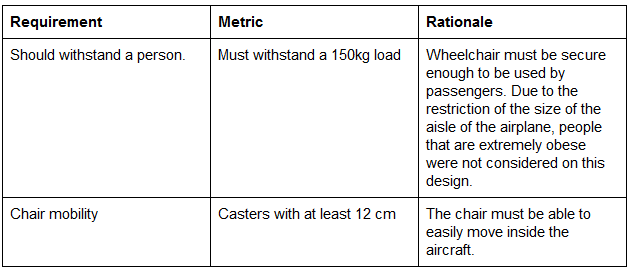
\includegraphics[scale=1]{images/functional_requirements_wheelchair_structure.png}
   \caption{Functional requirements for the wheelchair structure}
  \label{fig:fun_req_wheelchair_structure}
\end{figure}

\newpage

\begin{figure}[h!]
  \centering
     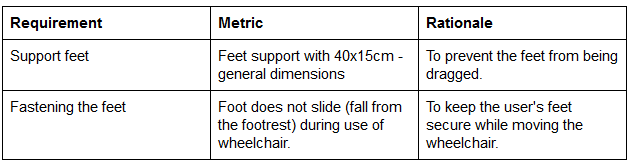
\includegraphics[scale=1]{images/functional_requirements_footrest.png}
   \caption{Functional requirements for the footrest}
  \label{fig:fun_req_footrest}
\end{figure}

\newpage

\begin{figure}[h!]
  \centering
     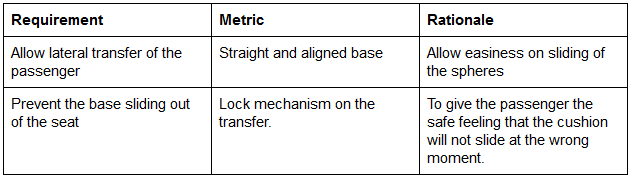
\includegraphics[scale=1]{images/functional_requirements_airplane_seat.png}
   \caption{Functional requirements for the airplane seat}
  \label{fig:fun_req_airplane_seat}
\end{figure}

\newpage

\subsection{Functional Constraints}

\subsection*{Wheelchair storage device}

\begin{list}{-}{}
  \item Due to FAA regulations and flight requirements the platform protecting the wheelchair must withstand 3 G's.
  \item The platfrom cannot damage the space or items within the space during its operation.
  \item The electronics will require a power source (battery) to perform some of its functions.
  \item The battery should satisfy the DOT’s Hazardous Materials Regulations (HMR; 49 CFR parts 100-185).
  \item The entire device needs to be approved as safe for air travel.
\end{list}

\subsection*{Wheelchair transfer mechanism}

\begin{list}{-}{}
  \item Due to FAA regulations and flight requirements every element that goes inside the cabin must withstand 6 G's.
  \item The redesigned aisle wheelchair must be as safe as the standard aisle wheelchair operated nowadays.
  \item The new aisle wheelchair has to operate in the restrained space of the airplane aisle.
  \item In case of turbulences, the wheels of the new aisle wheelchair must be blocked.
\end{list}

\subsection{Functional Assumptions}

\subsection*{Wheelchair storage device}

\begin{list}{-}{}
  \item Since the straps that are used to attach the wheelchair to the platform are the same as bus straps, wheelchair users are assumed to already be familiar with them. The use of this mechanism should provide them peace of mind since they already trust it in buses.
  \item The platform configuration changes (on the wheels to be moved or on the pallet to be stored) will be trigered by baggage handlers acting on an electric jack.
  \item Baggage handlers will be wearing their gloves with the RFID tag everytime that they handle a wheelchair and use our platform.
\end{list}

\subsection*{Wheelchair transfer mechanism}

\begin{list}{-}{}
  \item All aisle seats must have retractable armrest. It must allow the mechanism to slide without any obstacles in its way.
  \item The passenger will always be accompanied by a flight attendant to guarantee the safety of the passenger and to pull/push the aisle wheelchair.
  \item Tetraplegic passengers will always be accompanied by a travel companion/assistant. Because of regulation (ANAC) and their reduced autonomy, tetraplegic users are not allowed to fly alone.
  \item The airplane seat must withstand 19 G's during take-off and landing. This is what the FAA requires in order to make sure seats can withstand any type of accident happening during take-off or landing.
\end{list}

\subsection{Functional Opportunities}

\subsection*{Wheelchair storage device}

\begin{list}{-}{}
  \item Our platform must be intuitive to use. A baggage handler should know how to attch a wheelchair to the platform after a 15 mn training.
  \item Ideally the platform should have a braking system for the wheels to prevent it from moving too fast on a sloped surface. A braking device would allow handlers to have better control on the device.
\end{list}

\subsection*{Wheelchair transfer mechanism}

\begin{list}{-}{}
  \item Although we are desiging for a paraplegic user, it shall allow a tetraplegic user to be transferred from the aisle wheelchair to his/her seat with assistance. In this case, it should be a more pleasant experience since the assistant would not need to lift the tetraplegic user.
  \item The chest rest makes frontal transfer possible. Nowadays it cannot be done due to the current wheelchair dimensions.
  \item It reduces the risk associated to transfer because no one is carrying the disabled passenger. The chest rest is here to avoid human contacts that can be unpleasant and/or source of accidents.
  \item The chest rest allows paraplegic passengers to go to the restroom and use it.
\end{list}


\section{Physical Requirements}

\subsection*{Wheelchair storage device}

\begin{figure}[h!]
  \centering
     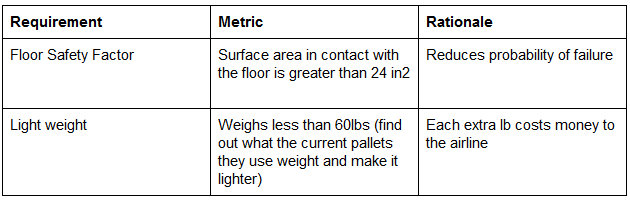
\includegraphics[scale=1]{images/physical_requirements_pallet.png}
   \caption{Physical requirements for the pallet}
  \label{fig:phy_req_pallet}
\end{figure}

\newpage

\begin{figure}[h!]
  \centering
     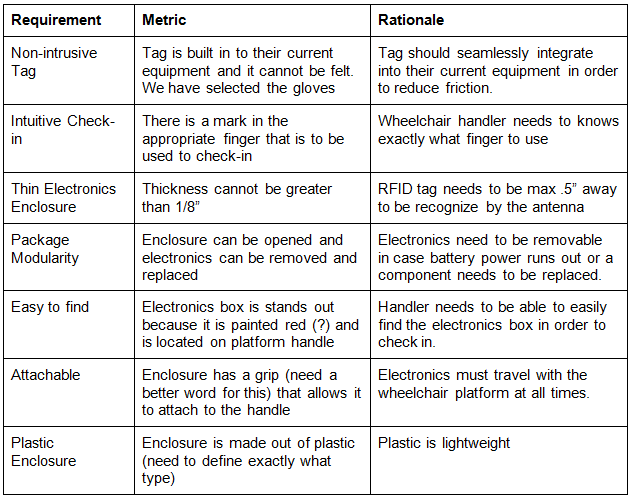
\includegraphics[scale=1]{images/physical_requirements_electronics.png}
   \caption{Physical requirements for the electronics}
  \label{fig:phy_req_electronics}
\end{figure}

\newpage

\begin{figure}[h!]
  \centering
     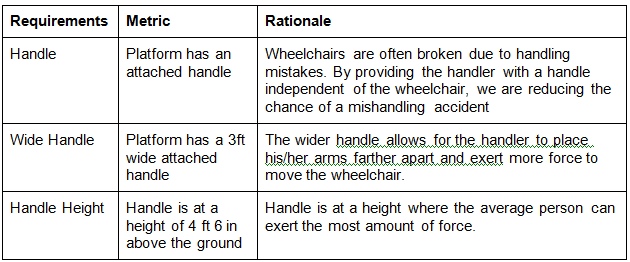
\includegraphics[scale=1]{images/physical_requirements_handle.png}
   \caption{Physical requirements for the handle}
  \label{fig:phy_req_handle}
\end{figure}

\newpage

\begin{figure}[h!]
  \centering
     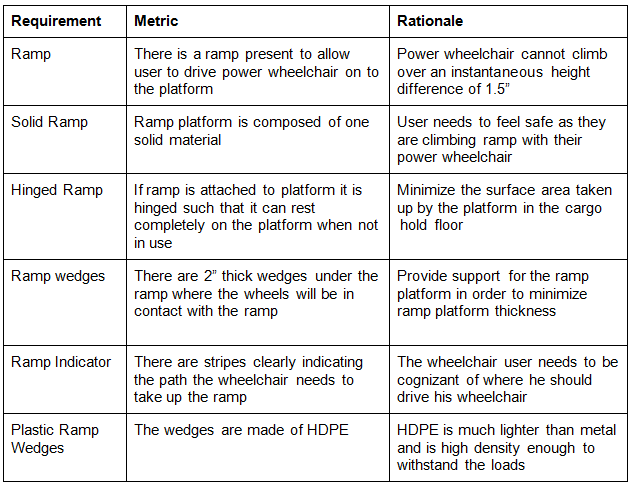
\includegraphics[scale=1]{images/physical_requirements_ramp.png}
   \caption{Physical requirements for the ramp}
  \label{fig:phy_req_ramp}
\end{figure}

\newpage

\subsection*{Wheelchair transfer mechanism}

\begin{figure}[h!]
  \centering
     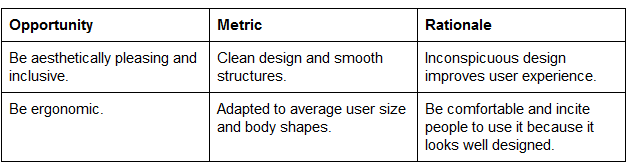
\includegraphics[scale=1]{images/physical_requirements_chest_rest.png}
   \caption{Physicall requirements for the chest rest}
  \label{fig:phy_req_chest_rest}
\end{figure}

\begin{figure}[h!]
  \centering
     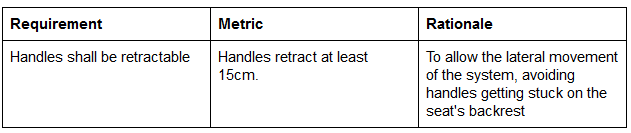
\includegraphics[scale=1]{images/physical_requirements_locomotion_mechanism.png}
   \caption{Physical requirements for the locomotion mechanism}
  \label{fig:phy_req_locomotion_mechanism}
\end{figure}

\begin{figure}[h!]
  \centering
     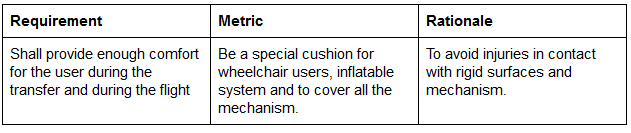
\includegraphics[scale=1]{images/physical_requirements_cushion.png}
   \caption{Physical requirements for the cushion}
  \label{fig:phy_req_cushion}
\end{figure}

\begin{figure}[h!]
  \centering
     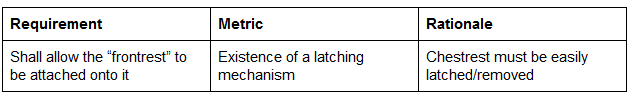
\includegraphics[scale=1]{images/physical_requirements_sliding_base.png}
   \caption{Physical requirements for the sliding base}
  \label{fig:phy_req_sliding_base}
\end{figure}

\newpage

\subsection{Physical Constraints}

\subsection*{Wheelchair storage device}

\begin{list}{-}{}
  \item The wheelchair load (more than 600 lbs for the heaviest wheelchairs) must be distributed over a minimum surface area of 8 in2 otherwise the stress experienced by the cargo hold floor will be too high and the floor may collapse. (All the details explaining how we got the 8 in2 figure are shown in appendix B).
  \item For th RFID identification system, the distance between the antenna and the tag must be as small as possible. The outer plastic surface covering the RFID antenna must be less than .25''.
  \item The box that encloses all the electronics must be very light weight (less than 3 oz).
  \item Power wheelchairs cannot climb an angle steeper than 6 degrees so the must inclination must be below this metric.
\end{list}

\subsection*{Wheelchair transfer mechanism}

\begin{list}{-}{}
  \item The width of the aisle (19.75'' in Embraer jets E175) limits the size of the aisle wheelchair.
  \item The new aisle wheelchair must be less than or equal to current aisle wheelchairs which weigh approximately 35 lbs.
\end{list}

\subsection{Physical Assumptions}

\subsection*{Wheelchair storage device}

\begin{list}{-}{}
  \item The ramp has to be modular. It is an attachment, not the platform itself because wheelchairs shoud not be stored at a 6 degree angle during a long flight. 
  \item The ramp has to be removed once used otherwise it would take too much space in the cargo hold.
\end{list}

\subsection*{Wheelchair transfer mechanism}

\begin{list}{-}{}
  \item We assume that the average wheelchair passenger using our transfer mechanism will have an average weight of 180 lbs.
  \item If disabled passengers have the opportunity to use the new redesigned aisle wheelchair to go to the restroom, we assume that this restroom is accessible and must have lateral grab bars.
\end{list}

\newpage

\subsection{Physical Opportunities}

\subsection*{Wheelchair storage device}

\begin{list}{-}{}
  \item The handle that enables baggage handlers to move the platform should be ergonomic. They should be covered by an ergonomic sleeve made of material such as silicon in order to increase comfort of pushing the platform around.
  \item The ramp should be attached to the platform in order to reduce the number of parts the airport personnel needs to handle.
  \item Having a hinged ramp serves double purpose. It can be used as a ramp and also as a stopper in case the wheelchair unstraps. It is here to increase user's peace of mind.
\end{list}

\subsection*{Wheelchair transfer mechanism}

\begin{list}{-}{}
  \item Wheelchair transfer from the passenger's wheelchair to the new aisle wheelchair will happen once the passenger has driven his/her mobility device on top of the platform. This way, baggage handlers do not manipulate the wheelchair at all. They only touch the platform. This should provide piece of mind to our user.
  \item Wheelchair users that are overweight should feel more comfortable in our redesigned aisle wheelchair because there is more support on the side.
\end{list}

